\chapter{Introduzione}
\label{chap:introduzione}

\section{Programma del corso di Chimica}
\label{sec:chimica}

\begin{itemize}
\item Definizioni e calcoli stechiometrici
\item La struttura dell'atomo
\item La tavola periodica degli elementi e le proprietà periodiche
\item Il legame cimico: teorie e tipologie. interazioni deboli. VSEPR e geometrie molecolari
\item Leggi dei gas
\item Termodinamica chimica
\item Equilibri chimici: acido-base e solubilità
\item Elettrochimica
\item Proprietà colligative
\end{itemize}

\section{La chimica}
\label{sec:chimdef}
\begin{defi}
  La chimica è la scienza che studia la composizione, la struttura e le trasformazioni della \underline{Materia}:\\
  La \underline{Materia}
  \begin{enumerate}
  \item Composizione (\texttt{analisi qualitativa e quantitativa})
  \item Struttura-proprietà, ad esempio, diamante-grafite
  \item Modellizzazione e progettazione
  \end{enumerate}
  Le trasformazioni della \underline{Materia}
  \begin{enumerate}
  \item Corrosione, ad esempio ferro e ruggine
  \item Combustione, ad esempio le sorgenti di energia
  \item Sintesi, ad esempio farmaci, pigmenti, nanomateriali, polimeri, \dots
  \end{enumerate}
\end{defi}
\begin{center}
  \Tree [.Universo [.Materia Ciò\ che\ occupa\ \underline{spazio}\ e\ ha\ \underline{massa} ]
  [.Energia Capacità\ di\ \underline{eseguire un lavoro} ] ]
\end{center}
Un \underline{sistema} è una porzione delimitata di spazio che rappresenta l'oggetto dello studio, mentre,
l'\underline{ambiente} è tutto ciò che sta attorno al sistema: l'insieme di {\color{red}sistema} e
{\color{blue}ambiente} costituisce {\color{blue}l'Universo}
\clearpage

\subsection{Gli stati della materia}
\label{sec:statidellamateria}

\begin{table}[ht!]
  \centering
  \begin{tabular}{lll}
    {\color{red}Solido}&{\color{blue}Liguido}&{\color{green}Gas}\\\hline
    Ha forma definta e volume & ha volume ma non forma & Non ha nè forma,\\
    proprio &  propria & nè volume proprio,\\
                       &&si espande in modo da\\
                       && riempire il contenitore\\
                       &&che lo contiene.\\\hline
  \end{tabular}
  \caption{Stati della materia}
  \label{tab:glistatidellamateria}
\end{table}

\begin{multicols}{2}[
  \subsection{Proprietà fisiche}
  \label{sec:propfisiche}
  La prioprietà che possono essere osservate e misurate {\color{red} SENZA} alterare la composizione della sostanza.
  Ad esempio:
  ]
  \begin{itemize}
\item colore;
\item punto di fusione e di ebollizione;
\item indice di rifrazione;
\item densità.
\end{itemize}
\end{multicols}
\subsection{Trasformazioni fisiche}
\label{sec:trasfisiche}
Trasformazioni che avvengono {\color{red} SENZA} alterare la composizione della sostanza, ad esempio:
\begin{itemize}
\item \textbf{ebollizione} di un liquido;
\item \textbf{fusione} di un solido;
\item \textbf{sciogliere} im solido in un liquido per ottenere una miscela omogenea (ovvero una
  {\color{blue}soluzione})
\end{itemize}

\subsection{Trasformazioni chimiche}
\label{sec:trasformazionichimiche}

Trasformazioni che avvengono ALTERANDO la natura della sostanze coivolte e portando alla formazione di nuovi compoti,
ad esempio: La combustione del metano.
\begin{center}
  Si parte da {\color{blue}metano} e {\color{blue}ossigeno} e si arriva a {\color{red}biossido di carbonio} e
  {\color{red}acqua}:
\end{center}
\begin{equation}
  \label{eq:esreagprod}
  \underbrace{{\color{blue}CH_4}+2{\color{blue}O_2}}_{\color{blue}reagente} \to \underbrace{{\color{red}CO_2}+2
  {\color{red}H_2O}}_{\color{red}prodotto}
\end{equation}
Al termine della trasformazione abbamo sostanze \textbf{diverse} da quelle di partenza.

\subsection{Miscela}
\label{sec:misc}

Combinazione di due o più sostanze pure
\begin{figure}[ht!]
  \centering
  \resizebox{5.5in}{!}{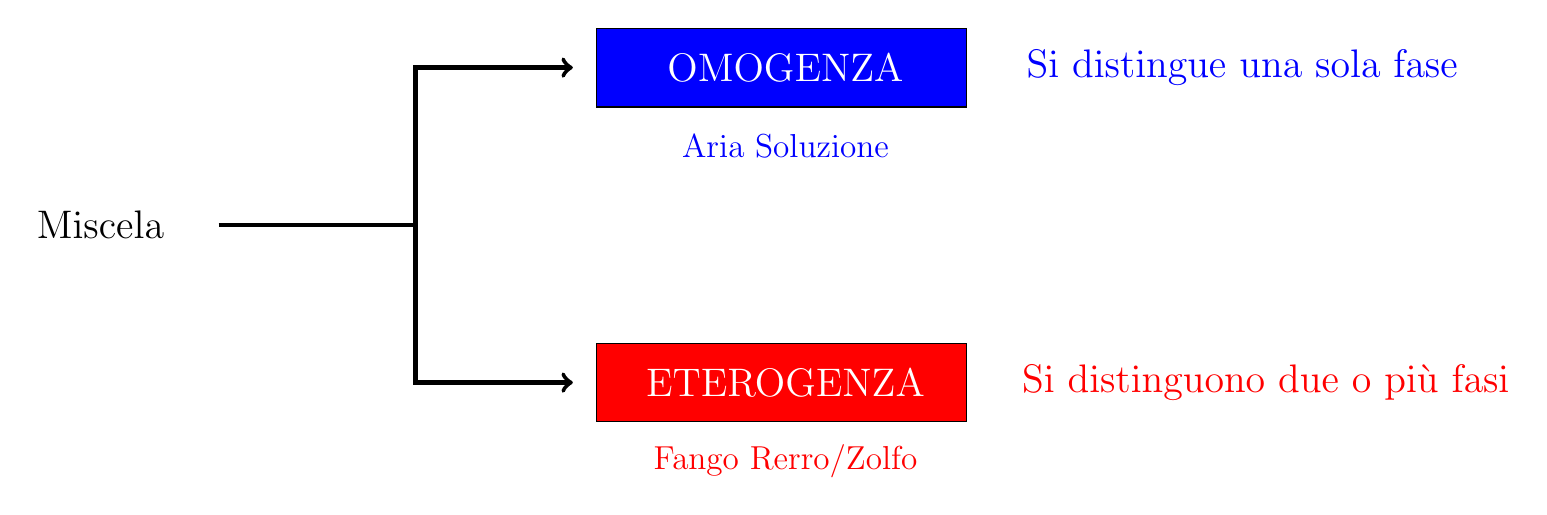
\begin{tikzpicture}
\node at (0,2) {\Large Miscela};
\draw[->,ultra thick] (1.5,2) -- (4,2) -- (4,4) -- (6,4);
\draw[fill=blue] (6.3,3.5) -- (6.3,4.5) -- (11,4.5) -- (11,3.5)  -- cycle;
\node[white] at (8.7,4) {\Large OMOGENZA};
\node[blue] at (14.5,4) {\Large Si distingue una sola fase};
\node[blue] at (8.7,3) {\large Aria Soluzione};

\draw[fill=red] (6.3,-.5) -- (6.3,.5) -- (11,.5) -- (11,-.5)  -- cycle;
\node[white] at (8.7,0) {\Large ETEROGENZA};
\draw[->,ultra thick]  (4,2) -- (4,0) -- (6,0);
\node[red] at (14.8,0) {\Large Si distinguono due o più fasi};
\node[red] at (8.7,-1) {\large Fango Rerro/Zolfo};
\end{tikzpicture}}
  \caption{Miscele}
  \label{fig:miscela}
\end{figure}
\section{La tavola periodica}
\label{sec:tavper}
\begin{defi}
  La tavola periodica degli elementi (o semplicemente tavola periodica) è uno schema che copnsente di ordinare
  gli elementi chimici sulla base loro numero atomico Z e del numero di elettroni presenti negli orbitali
  atomici s, p, d, f. Essa fu creata dal chimico e docente russo Dmitrij Ivanovič Mendeleev che pensò a questa
  soluzione per far studiare più comodamente i propri studenti, in un primo momento essa non fu ben vista
  dalla comunità scientifica ma poi una volta che si vide la comodità del suddetto sistema di rappresentazione
  vedendo pure il fatto che si potevano prevedere teorici elementi che andranno a ricoprire degli spazzi vuoti
  fu molto utile, ovviamente nel tempo fu modificata e stabilizzata rispetto all'originale previsto da
  Mendeleev, non fu l'unico a pensare a questa soluzione all'epoca, infatti, in modo indipendente il chimico
  tedesco Julius Lothar Meyer fece un qualcosa di simile.
\end{defi}
\begin{figure}[ht!]
  \centering
  \resizebox{5.5in}{!}{\input{img/tavPer.tikz}} 
  \caption{Tavola periodica degli elementi}
  \label{fig:tavper}
\end{figure}
\begin{itemize}
\item \underline{Elementi chimici}: sostenze pure che \underline{NON} possono essere decomposte ``separate'' in altre
  sostenze chimiche più semplici e sono costituite da atomi tutti ``uguali''
\item \underline{Simbolo atomico}: notazione sintetica costituita da uno o due lettere che rappresenta un determinato
  elemento. Spesso derivano dal nome latino dell'elemento.
\end{itemize}
\begin{table}[ht!]
  \centering
  \begin{tabular}{lll}
    \textbf{Simbolo}& \textbf{Nome} & \textbf{Etimologia nome}\\\hline
    Na & Sodio & Lat., \textit{natrium}, soda\\\hline
    Au & Oro & Lat., \textit{aurum}\\\hline
    S  & Zolfo & Lat., \textit{sulphur}\\\hline
    K  & Potassio & Ar., \textit{al-kali}\\\hline
    Sb & Antimonio & Lat., \textit{stibium}\\\hline
  \end{tabular}
  \caption{Simboli atomici}
  \label{tab:simatom}
\end{table}

\section{Composti chimici}
\label{sec:compchim}

\begin{defi}
  I composti chimici sono delle sostanze costituite da due o più elementi\\ $(H_2O,CaCO_3,H_2SO_4)$. Può essere di
  tipo \textbf{MOLECOLARE} (formato da molecole) o \textbf{IONICO} (costituito da ioni)
\end{defi}
\begin{center}
  \Tree[.Composti [.Molecola ] [.Ioni ] ]
\end{center}
\begin{itemize}
\item \underline{Molecola}: aggregato di atomi legati \texttt{covalentemente} ($H_2O,H_2,Cl_2,C_2H_5OH,\dots$)
\item \underline{Ioni}: Elementi che hanno perso elettroni e sono quindi carichi positivamente, \textit{\color{red}cationi}\\
  ($Li^+, Na^{2+},Al^{3+},\dots$) o acquistato elettroni e sono quindi carichi negativamente,
  \textit{\color{blue}anioni} \\
 eglinfo -B ($Cl^{-},Br^-,O^{2-},\dots$).
\end{itemize}
\clearpage

\subsection{Formula}
\label{sec:form}

\begin{defi}
  La formula è un rappresentazione di una sostanza mediante gli elementi presenti, indicante il numero atomico
  presente.
\end{defi}
\begin{table}[ht!]
  \centering
  \begin{tabular}{lll}
    \textbf{Formula Minima}&\textbf{Formula molecolare}&\textbf{Formula di struttura} \\\hline
    Indica gli elementi presenti & Indica gli elementi presenti & Indica anch come sono\\
    in un composto e i rapporti tra& in un composto e il loro & legati tra loro gli atomi\\
    questi, in termini dei più piccoli& numeri effettivi & di una molecola\\
    numeri interi\\
    $CH$ & $\begin{matrix}C_6H_6\\ C_2H_2\end{matrix}$& \chemfig{C(-[:0]H)(-[:90]H)(-[:180]H)(-[:270]H)}
                                                        \chemfig{*5(=-=-=-)} \chemfig{**4(------)}\\\\\hline
  \end{tabular}
  \caption[formminmolstruct]{Formula minima, molecolare e di struttura}
  \label{tab:formminmolstruct}
\end{table}

\subsection{Legge di conservazione della Massa o legge di Lavoisier}
\label{sec:legdiconse}
\colorbox{pink}
{
\begin{minipage}{.97\textwidth}
    <<IN UNA REAZIONE CHIMICA LA MASSA NON È NÉ CREATA NÉ DISTRUTTA, ESSA SI \underline{CONSERVA}>>
\end{minipage}
}
\begin{nota}
  Nel corso di vari esperimenti, Lavoisier dimostrò che la somma delle masse dei prodotti di una reazione chimica è
  uguale a quella dei reagienti.
  \begin{center}
    \ce{2HgO} \textrightarrow \ce{2Hg}+\ce{O2}\\
    \ce{AgNo3} + \ce{HCl} \textrightarrow \ce{HNO3}+\ce{AgCl}
  \end{center}
\end{nota}
\begin{defi}
  In un dato composto chimico i rapporti di massa degli elementi di cui esso è costituito sono
  \underline{costituiti}, indipendentemente dell'origine del composto o dal modo di preparazione
\end{defi}
\begin{description}
\item[\ce{NaCl} (cloruro di sodio)]
  \begin{itemize}
  \item Cloro 60.7\%
  \item Sodio 39.3\%
  \end{itemize}
\item[100g di \ce{NaCl} contengono]
  \begin{itemize}
  \item $60.7g$ di Cloro
  \item $39.3g$ di Sodio
  \end{itemize}
\end{description}

\section{Teorie sull'atomo}
\label{sec:atomo}
\textit{Dalla fine dell'otocento si sono succedute diverse teorie sulla struttura dell'atomo inteso come
  la parte più piccola di un elemento, il punto di non divisibilità, in cui non si può andare oltre nel separare il
  suddetto.}

\subsection{Teoria atomica di di Dalton}
\label{sec:dalton}
\begin{enumerate}
\item La matieria è costituita da atomi, particelle di materia indistruttibili e indivisibili.
\item Un elemento chimico è costituito da atomi tutti uguali tra loro. Cioè, un oggetto di rame, ad esempio,
  è costituito da soli atomi di rame. 
\item Elementi diversi sono costituiti da atomi diversi per volume, massa e proprietà. Ad esempio, l'idrogeno è un
  elemento molto piccolo ed è poco elettronegativo (l’elettronegatività è la tendenza di un atomo ad acquistare
  elettroni e quindi a caricarsi negativamente); invece l’ossigeno è molto più grande rispetto all’idrogeno ed è
  molto elettronegativo ({\it infatti l’ossigeno è l’elemento più elettronegativo dopo il fluoro che però è molto
    raro}).
\item Atomi uguali o diversi possono unirsi tra loro per formare composti chimici.
\end{enumerate}
\newpage
\subsection{Modello atomico di Thomson}
\label{sec:thomson}
\begin{defi}
  Nel 1897 Thomson identificò gli elettroni, particelle subatomiche con carica elettrica negativa e con massa 2000
volte più piccola della massa dell’atomo di idrogeno. La teoria atomica di Dalton, perciò, fu messa in discussione.
Thomson propose inoltre il primo modello di atomo in cui si facesse riferimento a particelle subatomiche, ovvero più
piccole dell’atomo.\\
Thomson ipotizzò che l'atomo fosse una sfera carica positivamente all'interno della quale erano disposti elettroni
che neutralizzassero la carica positiva.\\
Il modello di Thomson rappresentò un importante passo avanti, ma non convinceva del tutto: se c’erano delle
particelle subatomiche negative dovevano esserci anche delle subparticelle positive.
\end{defi}

\subsection{Modello atomico di Rutherford}
\label{sec:Rutherford}
\begin{defi}
  Gli studi di Rutherford sull'atomo si concentravano sulle radiazioni $\alpha$ (cioè atomi di elio caricati positivamente).
  Rutherford “bombardò” una sottilissima lamina d’oro (dello spessore di circa 200 atomi quindi 200u) con un
  fascio di radiazioni $\alpha$, mettendo un evidenziatore dietro la lamina.\\
  Alla prima osservazione sembrò che quasi tutte le particelle $\alpha$ attraversassero la lamina, ma osservazioni più
  accurate dimostrarono che un numero molto piccolo veniva deviato e che un numero ancora più piccolo veniva persino
  riflesso. Il fatto che quasi tutte le particelle attraversassero gli atomi di oro significava che non incontravano
  ostacoli. Le uniche due possibilità erano che incontrassero o spazi vuoti o elettroni. Di contro, le particelle
  che venivano deviate sfioravano i nuclei degli atomi e le particelle che venivano riflesse si scontravano con i
  nuclei degli atomi.\\
  Rutherford immaginò che l’atomo fosse come un piccolo sistema solare, un atomo planetario con un nucleo come sole
  ed elettroni come pianeti, dove ogni elettrone si muoveva lungo una precisa orbita.\\
  Ma De Broglie avanzò l’ipotesi che se l’elettrone si muoveva lungo una precisa orbita si poteva calcolare sia la
  velocità che lo spazio percorso.\\
  L’elettrone poteva quindi essere considerato come un’onda elettromagnetica. L’idea di elettrone onda fu accettata,
  ma a questo punto non si riusciva più a localizzarlo. Con il famoso Principio di Indeterminazione di Heisenberg,
  con cui dichiarava l’impossibilità di conoscere in pratica le caratteristiche del movimento dell’elettrone, si
  risolse il problema.
\end{defi}

\subsection{Modello atomico di Bohr}
\label{sec:bohr}
\begin{defi}
  I fisici del tempo di Eistein contrastavano molto Rutherford perché l’elettrone girando velocemente perde energia e quindi alla fine la sua carica elettrica doveva annullarsi. Inoltre sostenevano che la struttura dell’atomo non era planetaria. Ma Bohr (contemporaneo di Einstein), grazie l’uso degli spettri), ipotizzò un’altra struttura atomica in contrasto con quella di Rutherford.\\
Se si prende la luce bianca del sole e la si fa passare attraverso un prisma di vetro, si scompone e si può notare su una lastra fotografica: a questo punto si vede la scomposizione della luce bianca nei suoi colori. Ma Bohr studiò in particolare lo spettro dell’H2. Fu portato all’incandescenza e la luce fatta passare attraverso un prisma. Si notarono cinque bande di colori diversi con lo sfondo nero.\\
Bohr accettò l’ipotesi di Rutherford che l’atomo fosse formato da un nucleo (con all’interno i nucleoni) e da elettroni che si trovavano su livelli energetici. Questi poi furono chiamati orbite ma dato che l’elettrone (che è sia onda che particella) si muove intorno al nucleo con un moto impossibile da definire si deve parlare di possibilità, cioè di orbitale.\\
Secondo Bohr i livelli energetici sono quantizzati, cioè ogni livello energetico ha una quantità di energia diversa, per esempio la quantità di energia n=1 è maggiore di n=2. A mano a mano che ci si allontana dal nucleo, quindi, la quantita di energia diminuisce. Questa quantità di energia è detta Quanto. Precisamente il quanto di energia è definito come l’energia necessaria all’elettrone per far passare l’elettrone stesso da un livello energetico ad un altro. Se invece vogliamo far passare un elettrone da n=3 a n=1 bisogna togliere energia.\\
Bohr calcolò anche il raggio dell’orbità: r=53n(al quadrato) pm
\end{defi}

\section{L'atomo}
\label{sec:l'atomo}
\textit{L'atomo è la particella più piccola di un elemento che possiade tutte le caratteristiche chimiche
  dell'elemento. l'atomo è prevalentemente spazio vuoto (99.999\dots\%)}
\begin{tasks}
  \task protoni e neutroni sono nel nucleo (99.99\dots\% della massa totale dell'atomo)
  \task il numero di elettroni è uguale al numero di protoni
  \task gli elementi occupano lo spazio attorno al nucleo.
  \task è estremamemnte piccolo\dots Il numero di atomi presenti in un cucchiaino di acqua è 3 volte il numero di
  cucchiaini di acqua nell'Oceano Atlantico.
\end{tasks}

\subsection{Composizione atomica}
\label{sec:compatom}
\begin{table}[!ht]
  \centering
  \begin{tabular}{lclll}
    &Carica relativa&Carica assoluta&Massa assoluta & Massa relatva\\\hline
    \textbf{Protoni} & +1 & $+1.602\cdot 10^{-19}C$ & $1.673\cdot 10^{-27}Kg$ & 1.007 u.m.a\\\hline
    \textbf{Elettroni} & -1  & $-1.602\cdot 10^{-19}C$ & $9.109\cdot 10^{-31}Kg$ & 0.0005 u.m.a*\\\hline
    \textbf{Neutroni} & \multicolumn{2}{c}{\color{red}nessuna carica elettrica} & $1.675\cdots10^{-27} Kg$
                                    & 1.009 u.m.a.\\
    \hline
  \end{tabular}
  \caption{Composizione atomica}
  \label{tab:compatom}
\end{table}
*u.m.a. = unità di massa atomica; 1 u.m.a. = $1.6605665\cdot 10^{-24}g$

\subsection{Numero atomico, Z}
\label{sec:numatom}

Tutti gli \underline{\color{red} atomi} dello stesso \underline{\color{blue}elemento} hanno lo stesso numero di
{\color{green} protoni} nel \underline{nucleo}.
\begin{center}
  Il numero di protoni è chiamato: \underline{\color{green}NUMERO ATOMICO}\\
  Si indica con la lettera {\color{green}Z} maiuscola
\end{center}
Poichè un \textbf{atomo} è \underline{elettricamente neutrale}, il numero di {\color{green}protoni} è uguale
al numero di {\color{red}elettroni} che circondano il \textit{nucleo}.
\begin{center}
  \colorbox{green}{$N^o$ PROTONI} = \colorbox{red}{$N^o$ ELETTRONI}
\end{center}

\subsection{Numero di Massa, A}
\label{sec:num.massa,a}

Il \textbf{numero di massa} è la somma dei protoni e dei neutroni presenti nel nucleo dell'atomo.
\begin{center}
  {\color{blue}Numero di Massa (A)} = \textit{\color{red}$n^o$ protoni} + \textit{\color{green}$n^o$ neutroni} 
\end{center}
Un atomo di boro può avere: ${\color{blue}A} = 5{\color{red}p} +5{\color{green}n}=10uma$.
\begin{figure}[ht!]
  \centering
  \resizebox{3.5in}{!}{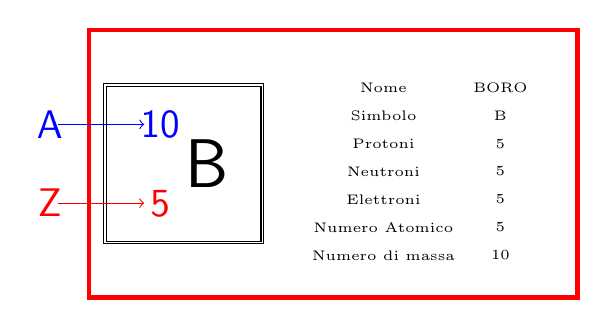
\begin{tikzpicture}
\draw[red,ultra thick] (-.2,-.2) -- (-.2,3.2) -- (6,3.2) -- (6,-.2) -- cycle;
\draw[double] (0,.5) -- (0,2.5) -- (2,2.5) -- (2,.5) -- cycle; 
\node[font=\Huge] at (1.3,1.5) {\textsf{B}};
\node[font=\Large,blue] at (.7,2) {\textsf{10}};
\node[font=\Large,red] at (.7,1) {\textsf{5}};
\node[font=\Large,blue] at (-.7,2) {\textsf{A}};
\node[font=\Large,red] at (-.7,1) {\textsf{Z}};
\draw[->,red] (-.6,1) -- (.5,1);
\draw[->,blue] (-.6,2) -- (.5,2);
 \matrix [nodes={font=\tiny,minimum size=1mm}] at (4,1.4)
  {
    \node {Nome}; & \node{BORO};  \\
    \node {Simbolo}; & \node{B};  \\
    \node {Protoni}; & \node{5};  \\
    \node {Neutroni}; & \node{5};  \\
    \node {Elettroni}; & \node{5};  \\
    \node {Numero Atomico}; & \node{5};  \\
	\node {Numero di massa}; & \node{10};  \\
  };
\end{tikzpicture}} 
  \caption{Esempio di numero di massa e di numero atomico}
  \label{fig:es}
\end{figure}

\section{Isotopi}
\label{sec:isotopi}
Atomi delo stesso elemento (stessa {\color{red}Z}) ma aventi diverso numero di massa ({\color{blue}A})
\clearpage
\begin{table}[th!]
  \centering
  \begin{tabular}{ccc}
    \ce{^{6}_3 Li}&&\ce{^{7}_3Li}\\\hline
    Litio & Nome & litio \\\hline
    Li & Simbolo & Li\\\hline
    3 & Protoni & 3\\\hline
    3 & Neutroni & 4\\\hline
    3 & Elettroni & 3\\\hline
    3 & Numero Atomico & 3\\\hline
    6 & Numero di massa & 7\\\hline
  \end{tabular}
  \caption{Esempio della differenza di Isotopi tra il liteo \ce{^{6}_3 Li} e il \ce{^{7}_3Li}}
  \label{tab:esIso}
\end{table}
\begin{oss}
  Gli {\color{orange}isotopi} di un elemento, sebbene abbiamo \underline{masse differenti}, non differiscono nel
  \textbf{comportamento chimico} perché hanno lo stesso numero di {\color{green}protoni} (numero atomico) e quindi
  lo stesso numero di {\color{red}elettroni}.
\end{oss}

\subsection{Isotopi dell'idrogeno}
\label{sec:IsoIdrogen}

L'idrogeno (\ce{H}) è formato da tre isotopi che possiedono ciascuno un {\color{red}protone} ma differisono per il
numero di \textbf{\color{gray}neutroni}
\begin{table}[th!]
  \centering
  \begin{tabular}{ccc}
    \ce{^1_1H}&\ce{^2_1H}&\ce{^3_1H}\\\hline
    Idrogeno & deuterio & trizio\\\hline
    Protio & Idrogeno pesante &\\\hline
  \end{tabular}
  \caption{Isotopi dell'idrogeno}
  \label{tab:isotopidro}
\end{table}
\begin{oss}
  Nel caso del trizio è radioattivo
\end{oss}

\subsection{Isotopi del carbonio}
\label{sec:isocarbon}

Il carbonio è formato da tre isotopi che possiedono ciascuno sei {\color{red}protoni} ma differiscono per il numero
di {\color{gray}neutroni}.
\begin{table}[th!]
  \centering
  \begin{tabular}{ccc}
    \ce{^{12}_6C}&\ce{^{13}_6C}&\ce{^{14}_6C}\\\hline
    carbonio-12 & carbonio-13 & carbonio-14\\\hline
    6 protoni & 6 protoni & 6 protoni\\
    6 neutroni & 7 neutroni & 8 neutroni\\\hline
    (98.98\%) & (1.01\%) & ($1/{10^{12}}$ atomi di C)\\
    && Radiattivo\\\hline
  \end{tabular}
  \caption{isotipi del carbonio}
  \label{tab:isocarbon}
\end{table}

Il \ce{^{14}_6C} è radeattivo (instabile) con un tempo di dimezzamento di 5700 anni.Lo si usa per datare i reperti
archeologici.\\
Come conseguenza dell'esistenza degli isotopi, la massa di un insieme di atomi ha un valore medio.
\begin{center}
  \colorbox{green}{Massa Media} = \colorbox{red}{Massa Atomica}
\end{center}
Ad esempio, Il Boro è 20\% \ce{^10B} e 80\% \ce{^11B} ha una abbondanza terrestre pari all'80\%.
\section{Massa atomica}
\label{sec:massatom}

\begin{itemize}
\item Determinata sperimentalmente risulta inferiore rispetto alla somma dei costituenti. Il ``difetto di massa''
  è dovuto all'energia che si sviluppa quanto si formano i nuclei.
\item La massa degli atomi (\ce{10^{-24}-10^{-22} g}) è troppo piccola per essere espressa in kg o g. Si ricorre
  a una massa relativa.
\item Definisce la massa di un elemento rispetto a unatomo di un altro elemento.
\item Ad esempio, un atomo di \ce{O} è circa 16 volte più pesante di una atomo di \ce{H}.
\end{itemize}
\begin{itemize}
\item Occorre definire un elemento come standard rispotto al quale vengono misurati tutti gli altri.
\item Per convenzione la massa del \ce{^12C} è stata posta esattamente uguale a 12 u.m.a.
\item Perciò un u.m.a. è uguale a $\frac{1}{12}$ della massa del \ce{^12C}
\end{itemize}

\section{Come contare gli atomi?}
\label{sec:contatomi}

Il carbonio brucia all'aria \ce{C_{(s)} + O_{(g)}\to CO_{2(g)}}
\begin{center}
  {\color{red}1} atomo \ce{C} + {\color{red}1} molecala \ce{O2} producono {\color{red}1} molecola \ce{CO2}\\ 
  {\color{red}100} atomo \ce{C} + {\color{red}100} molecala \ce{O2} \textrightarrow{} {\color{red}100} molecola
  \ce{CO2}\\ 
  {\color{red}2000} atomo \ce{C} + {\color{red}2000} molecala \ce{O2} \textrightarrow{} {\color{red}2000} molecola
  \ce{CO2}\\
  \dots
\end{center}
\begin{att}
  Questi numeri corrispondono alle quantità in peso estremamaente ridotte, non utilizzabili in laboratorio.
\end{att}
{\color{red} Si introduce una ``unità di misura'' conveniente che permette di utilizzare pesi convenienti nella
  pratica di laboratorio:}
\begin{center}
  \ce{N atomi C + N molecole O2 \to N molecole CO2}
\end{center}

\section{Macroscopico e Microscopico}
\label{sec:macroemicro}

\begin{description}
\item[Macroscopico] tutto ciò che si può conoscere da una diretta osservazione delle proprietà fisiche delle materie
  e dele sue trasformazioni.
\item[Microscopico] Il livello atomico, costituito da atomi e molecole, così piccole da non essere visibile ad
  occhio nudo o da strumenti di ingrandimento non elettronici.
\end{description}
\colorbox{pink}
{
\begin{minipage}{.97\textwidth}
  La \textbf{MOLE} ci permette di collegare il livello microscopico con il livello macroscopico, in cui abbiamo a
  che fare con la quantità di sostanza che possono essere pesata e maneggiate.
\end{minipage}
}

\subsection{La mole}
\label{sec:lamole}
Unità per la quantità di materia
\begin{itemize}
\item 1 mole (mol) di qualsiasi sostanza contiene un numero di particelle (atomi, molecole, ioni, elettroni,\dots)
  pari al numero di Avogadro (\ce{N_A=6.022 x 10^{23}})\footnote{Una mole è quella quantità di ``qualcosa'' che
    corrisponde a 602.214.179.000.000.000.000.000 unità}.
\item 1 mole è la quantità di sostanza che contiene tante particelle (atomi, molecole) quante sono contenute in 12.0g
  di \ce{^12C}.
\end{itemize}
\begin{notab}
  se si prendesse un numero di palline da ping-pong pari al numero di Avogadro, e le si disponesse in modo omogeneo
  sulla superficie terrestre, si raggiungerebbe un altezza di 50 chilometri, ovvero più di 6 volte l'altezza
  dell'Everest.
\end{notab}
\clearpage
\begin{figure}[ht!]
  \centering
  \resizebox{3.5in}{!}{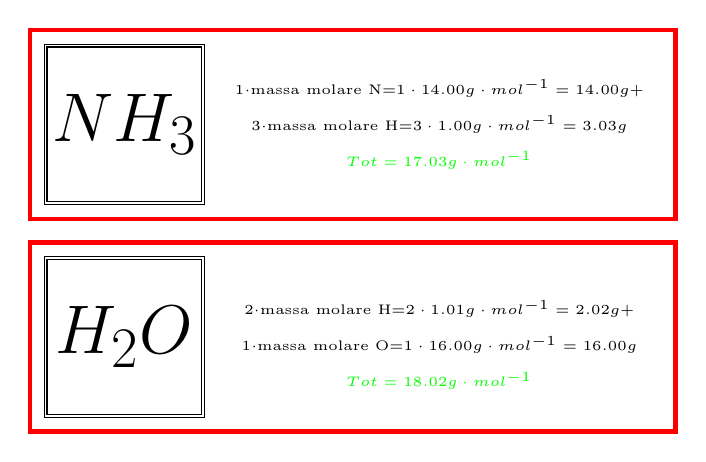
\begin{tikzpicture}
\draw[red,ultra thick] (-.2,0.3) -- (-.2,2.7) -- (8,2.7) -- (8,0.3) -- cycle;
\draw[double] (0,.5) -- (0,2.5) -- (2,2.5) -- (2,.5) -- cycle; 
\node[font=\Huge] at (1.0,1.5) {\textsf{$H_2O$}};
 \matrix [nodes={font=\tiny,minimum size=1mm}] at (5,1.4)
  {
    \node {$2\cdot$massa molare H=$2\cdot1.01g\cdot mol^{-1}=2.02g+$};   \\
    \node {$1\cdot$massa molare O=$1\cdot16.00g\cdot mol^{-1}=16.00g$};  \\
	\node {$\color{green}Tot=18.02g\cdot mol^{-1}$};  \\
  };

\draw[red,ultra thick] (-.2,3) -- (-.2,5.4) -- (8,5.4) -- (8,3) -- cycle;
\draw[double] (0,3.2) -- (0,5.2) -- (2,5.2) -- (2,3.2) -- cycle; 
\node[font=\Huge] at (1.0,4.2) {\textsf{$NH_3$}};
 \matrix [nodes={font=\tiny,minimum size=1mm}] at (5,4.2)
  {
    \node {$1\cdot$massa molare N=$1\cdot14.00g\cdot mol^{-1}=14.00g+$};   \\
    \node {$3\cdot$massa molare H=$3\cdot1.00g\cdot mol^{-1}=3.03g$};  \\
	\node {$\color{green}Tot=17.03g\cdot mol^{-1}$};  \\
  };
\end{tikzpicture}} 
  \caption{Esempio di massa Molare}
  \label{fig:esmol}
\end{figure}

Le {\color{red}formule chimiche} sono scritture simboliche che contengono tutta l'informazione
{\color{blue}qualitativa} (quali tipi di atomo) e {\color{purple}quantitativo} (quanti atomi) necessaria a
descrivere la composizione atomca della sostanza.
\begin{center}
  \Tree[.\ce{CO2} [.Visione\ molecolare ] [.Visione\ molare ] ]
\end{center}
\begin{description}
\item[Visione Molecolare] Una molecola (44.01 uma) contiene:\\
  1 atomo \ce{C} (12.01 uma)\\
  2 atomo \ce{O} ($2\times 16.00=32.00uma$)
\item[Visione Molare] 1 mol di molecola (44.01g) contiene:\\
  1 mol di atomi \ce{C} (12.01g)\\
  2 mol di atomi \ce{O} ($2\times 16.00g=32.00g$)
\end{description}

\begin{ess}
  \label{ess:esMolEnumDiMol1}

Calcolare la massa molare dell'acido acetico sapendo che ha formula minima \ce{CH2O} e che il numero di atomi di
ossigeno presenti per molecole è uguale a 2.
\begin{center}
  \textit{masse molari atomiche: $H=1.01g\cdot mol^{-1};C=12.01g\cdot mol^{-1};O=16.00g\cdot mol^{-1}$}
\end{center}
\begin{tasks}
  \task Calcolare la formula molecolare, considerando che ci sono 2 atomi di ossigeno (\ce{O}) per molecola, la
  formula molecolare si ricava moltiplicando per 2 i coefficienti di quella minima.
  \begin{center}
    \ce{(CH2O) \cdot 2 \to C2H4O2}
  \end{center}
  \task Calcoliamo il contributo di ciascun elemento:
  \begin{eqnarray*}
    Carbonio=2mol\cdot 12.01\frac{g}{mol}=24.02g;\\
    Idrogeno=4mol\cdot 16.00\frac{g}{mol}=4.04g;\\
    Ossigeno=2mol\cdot 16.00\frac{g}{mol}=32.00g
  \end{eqnarray*}
  \task Calcoliamo il contributo di ciascun elemento:
  \begin{center}
    $MM_{Acido acetico}=(24.02g+4.04g+32.00g)\cdot mol^{-1}=60.06g\cdot mol^{-1}$
  \end{center}
\end{tasks}
\subsubsection{Risultato}
\label{sec:esMolEnumDiMolris1}

\begin{table}[ht!]
  \centering
  \begin{tabular}{lc}
    Massa molare & $60.06g\cdot mol^{-1}$\\\hline
    Massa di una molecola & $60.60 u.m.a.$\\\hline
  \end{tabular}
  \caption{risultato}
  \label{tab:risesmol1}
\end{table}
\end{ess}
\clearpage
\begin{ess}
 Calcolare quante moli sono contenute in 30.03g di acido acetico (\ce{C2H4O2}).
\begin{tasks}
  \task Calcolare la massa molare dell'acido acetico:
  \begin{eqnarray*}
    Carbonio=2mol\cdot 12.01\frac{g}{mol}=24.02g\\
    Idrogeno=4mol\cdot 1.01\frac{g}{mol}=4.04g\\
    Ossigeno=2mol\cdot 16.00\frac{g}{mol}=32.00g\\
    MM_{Acido acetico}=24.02g+4.04g+32.00g=60.06g
  \end{eqnarray*}
  \task Calcoliamo il numero di moli contenute nella quantità data:
  \begin{eqnarray*}
    mol_{Acido acetico} = \frac{\text{massa acido acetico (g)}}{\text{Massa Molare Acido acetoco } \left(\frac{g}{mol}
    \right)} =\frac{30.03g}{60.06\frac{g}{mol}}=0.50mol
  \end{eqnarray*}
\end{tasks} 
\end{ess}
\begin{ess}
 \label{ess:esNmoli}

Calcolare quante moli sono contenute in $42.05g$ di carbonio di calcio (\ce{CaCO3}), sapendo che le masse molari
atomiche sono \ce{Ca=40.08g\cdot mol^{-1}}, \ce{C=12.01g\cdot mol^{-1}} e \ce{O = 16.00 g\cdot mol^{-1}}.
\begin{tasks}
  \task Calcolare la massa molare (MM) del carbonato di calcio:
  \begin{eqnarray*}
    Calcio=1mol\cdot 40.08\frac{g}{mol}=40.08g\\
    Carbonio=1mol\cdot 12,01\frac{g}{mol}=12.01g\\
    Ossigeno=3mol\cdot 16.00\frac{g}{mol}=48.00g\\
    MM_{CaCO_3}=40.08g+12.01g+48.00g=100.09
  \end{eqnarray*}
  \task Calcoliamo il numero di moli contenute nella quantità data:
  \begin{equation*}
    mol_{CaCO_3}=\frac{\text{massa } CaCO_3(g)}{\text{Massa Molare } CaCO_3\left(\frac{g}{mol}\right)}=\frac{42.05g}{100.09\frac{g}{mol}}=0.42mol
  \end{equation*}
\end{tasks} 
\end{ess}
